\chapter{大尺度脑电研究的谱异质同构质量指标}

\section{引言}
发展集成的脑电数据处理分析流水线平台的一个挑战是最初的预处理阶段,这一阶段需要去掉脑电伪差但也有可能去除与大脑活动有关的脑电信号。 存在脑电预处理流水线平台包括: Prep\citing{bigdely-shamlo_prep_2015}、Automagic\citing{pedroni2019automagic}、HAPPE\citing{gabard2018harvard}、Lossless\citing{lossless-eeg_2020}和Autoreject\citing{jas2017autoreject}等等。 这些都依赖于要信号的质量指标,根据该指标可以一导联信号或者一段信号去除伪差或者进行矫正。 脑电信号要经过滤波和独立成分分析基于的伪差成分去除。 当评估脑电预处理流水线时,我们遇到多通道$\log$谱相互平行的问题,即如图\ref{Fig 1(A)}所示每个电极上所有谱是相互平行的。 这意味着头表的谱地形图在不同频率之间非常相似,意味着神经源空间对所有频率存在着在相近位置上活动的偶极子,脑电的实际源可能因为去除过多的伪差而难以识别,违背了不同频率下不同神经源共振模式的事实\citing{hacker2017frequency}。 在本章中,我们提出一种质量指标,能够评估脑电频谱有多大程度上在电极之间是相互平行的。

\section{研究背景}
神经电生理大数据的出现需要相应的批量自动化处理程序\citing{bigdely-shamlo_prep_2015}。 这些程序的例子是自动化的伪差去除\citing{jas2017autoreject},自动的正演模型求解\citing{huang2019realistic,vorwerk2018fieldtrip},自动的溯源分析\citing{niso2019brainstorm,weinstein2001biopse}以及统计分析。 最重要的工作是对这些自动化的程序进行质量控制(quality control, QC),能够代替人脑劳动对自动化处理程序进行监督\citing{jas2018reproducible}。 利用如脑电等电生理技术手段高的时间分辨率和频谱分析技术,人们希望刻画到神经源连接的空间模式,它可以作为脑认知功能和精神紊乱的潜在生物标记物\citing{friston2011functional,jirsa2007handbook,mars2018connectivity,schoffelen2009source}。 自动化数据分析的第一步是筛选脑电脑磁数据、去除伪差等等。 然后更通常的是,我们对时域的波形进行谱估计输出交叉谱,交叉谱能够代表大脑活动的全部动力学信息\citing{nolte2019mathematical,siegel2012spectral}。 最后,一种溯源分析方法能够转换头表空间的交叉谱到神经源空间\citing{bosch20013d}。 尽管已经存在一些自动的脑电脑磁数据预处理程序,例如Automagic\citing{pedroni2019automagic}、autoreject\citing{jas2017autoreject}、PREP\citing{bigdely-shamlo_prep_2015}、HAPPE\citing{gabard2018harvard}、APP\citing{da2018automatic}和加拿大布鲁克大学心理学院研究的lossless,尚没有一个能够检查伪差去除后的频域失真。 尽管在实际中我们难以知道脑电脑磁数据无噪声信号的集标准,但可以认为应用越多越复杂的伪差去除程序,也有可能去除与脑活动相关的信号。 在结合强力的算法进行伪差去除后得到的脑电脑磁好看的波形可能离大脑活动的内在动力学相差较远或者改变了大脑的源活动的连接空间模式。
\begin{figure}
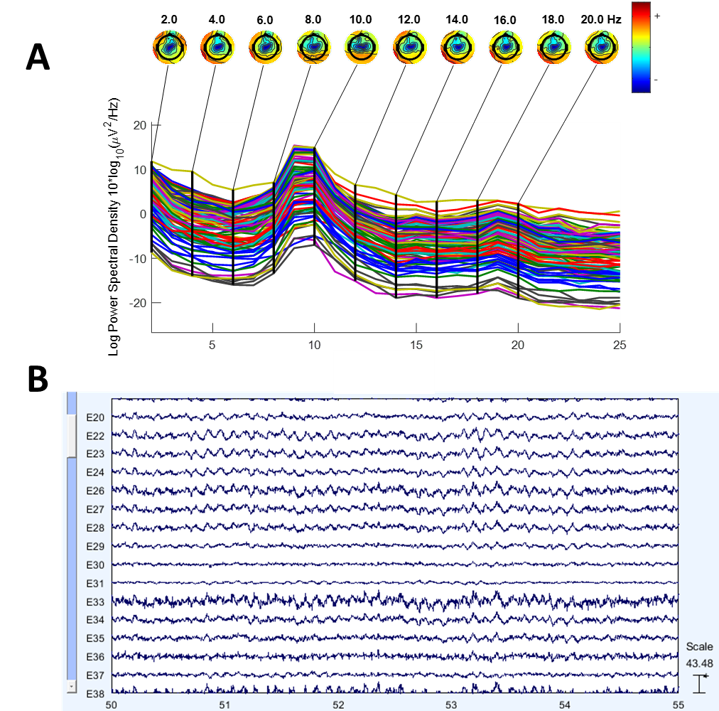
\includegraphics[width=15cm]{pic/palos/issue.png}
\caption{多通道功率谱同构问题示例。 A.被试数据经Automagic\citing{pedroni2019automagic}预处理后EEGLAB画出的功率谱, 不同颜色的曲线代表不同电极的功率谱,可以看出功率谱曲线高度平行,不同频率下的谱地形图分布很相似;B.经Automagic预处理后被认为是干净的脑电数据波形。}
\label{fig1}
\end{figure}

然而,电生理神经成像将无创地记录到的脑电脑磁数据视为大脑活动信号,大脑信号的微弱和传感器的敏感更容易在得到的脑电磁记录中混有各种各样的噪声,采集的数据数据常不是很好看。 无论脑电脑磁数据经过了怎样的预处理,在进一步分析动力学或者源活动之前的必要一步是对头表上估计得到的频谱进行质量分析。 我们发现$\log$转换之后的频谱在所有电极之间是相互平行的,即Parallel LOg Spectra (PaLOS) 问题。 如图\ref{fig1}所示,较短频率间隔上的谱地形图呈现稳定相似的空间模式,这可能表明神经源偶极子的震荡情况是基本不变的,与大脑具有依赖于频域高度震荡的动力学信息这一认识相背离\citing{cabral2017functional,deco2011emerging}。 也有研究认为大脑连接更可能依赖于频率呈现不同的模式而不是静态固定的\citing{chang2010time,foster2015intrinsic,hacker2017frequency,thompson2015frequency}。

在本章中,我们提出用第一个共同的主要成分\citing{trendafilov2010stepwise}在交叉谱数据中所有频率上占的比例作为判定伪差去除后的脑电脑磁数据是否具有PaLOS现象的质量准则。 直观地推理,如果多通道功率谱在所有频率上电极之间是相互平行的,所有通道的谱曲线就是一个共同的主要尺度加减不同尺度平移后的结果。 多通道功率谱相互平行这个单变量的问题可以推广到交叉谱的多变量的情况, 所有频率的交叉谱由共同主要交叉谱空间模式的尺度变换版本合成且其中一个具有解释全部方差的最大成份。

为了验证第一个共同的主要成分是合适的质量准则,我们需要考虑一些可能人为地通过插值增加通道之间相关性共线性而引入的PaLOS问题,例如脑电的参考过程\citing{hu_how_2018},使用独立成分分析的去除过多的成分,插值修复坏道,和眼电的回归等等。 

\section{研究方法}
\subsection{谱同构模型}
图\ref{fig1}(A)表示了多通道功率谱同构的现象,多通道功率谱在$\log_{10}$上相互平行,可以表示为
\begin{equation}\label{eq1}
\log_{10}\mathbf{p}^\omega=\mathbf{c}+\log_{10}\bar{\mathbf{p}}^\omega
\end{equation}
这里$\mathbf{p}^\omega$指的是在频率点$\omega$下所有电极上的功率谱,$\bar{\mathbf{p}}$是单频率点下所有电极上功率谱平均值,$\mathbf{c}$是一列由对应到各个电极上的偏差常数组成的向量。

在$\log_{10}$上相互平行的功率谱,转换到自然尺度上,就是单个频率点上成比例的功率谱,对于逐个电极$i\in[1,...,N_e]$,我们可以表示为
\begin{equation}\label{eq2}
\begin{split}
\mathbf{p}^\omega& =\mathbf{10^c}\bar{p}^\omega\\
p_i^\omega& =10^{c_i}\bar{p}^\omega
\end{split}
\end{equation}

因为谱的方差意义,考虑对单频率下大小为所有电极$\times$所有数据段的傅里叶系数矩阵进行主成分分析,记负载(loadings)矩阵为$\mathbf{L}^\omega$,记白化(whitening)矩阵为$\mathbf{\Gamma}^T=[\mathbf{\gamma}_1,...,\mathbf{\gamma}_{N_e}]$,逐个电极上的功率谱可记为
\begin{equation}\label{eq3}
\begin{split}
\mathbf{L}^\omega& =\mathbf{\Gamma}\mathbf{D^{1/2}}^\omega\\
p_i^\omega& =\mathbf{\gamma}_i^T\mathbf{D}^\omega\mathbf{\gamma}_i
\end{split}
\end{equation}
这里$\mathbf{\Gamma}$是正交阵,服从$\mathbf{\Gamma}\mathbf{\Gamma}^T=\mathbf{I}$,$\mathbf{D}$是由特征值平方组成的对角阵。通过主成分分析,我们不妨把多通道电极功率谱在自然尺度上成比例转换为傅里叶系数的负载矩阵第一个电极上对应的特征值占优。

考虑到同构的多通道功率谱是多通道电极之间交叉谱的对角元,记交叉谱为$\mathbf{S}^\omega$,对所有频率点$\omega\in[1,...,N_\omega]$下的大小为所有电极$\times$所有数据段的傅里叶系数矩阵都进行主成分分析。 因为多通道功率谱同构是所有电极的功率谱关于频率的曲线相互平行,我们可推断不同频率下多通道电极之间的交叉谱矩阵具有相似的主成分空间\citing{boik1988common,krzanowski1984principal},我们采用共同的主成分分析的方法\citing{trendafilov2010stepwise}得到
\begin{equation}\label{eq4}
\mathbf{S}^\omega=\mathbf{\Gamma}\mathbf{D}^\omega\mathbf{\Gamma}^T
\end{equation}
这里$\mathbf{\Gamma}$不随频率变化,$\mathbf{D}^\omega$作为由交叉谱矩阵的特征值平方组成的对角矩阵随频率变化。 \eqref{eq4}是从单变量的多通道电极功率谱同构到多变量的多通道电极交叉谱同构模型的推广。图\ref{fig2}是多通道电极交叉谱在所有频率下的示意图,图\ref{fig1}A中所有电极的功率谱在$\log_{10}$尺度上关于频率的平行曲线可以看作图\ref{fig2}中每一个频率点下所有电极交叉谱矩阵的对角线的值随频率变化的曲线相互之间成比例。

\begin{figure}
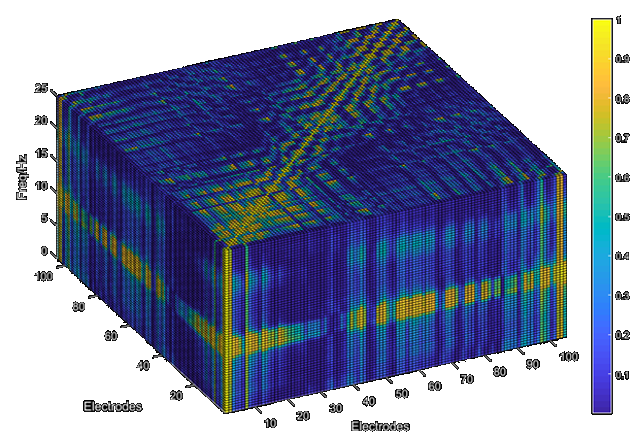
\includegraphics[width=15cm]{pic/palos/spectratensor.png}
\caption{多个频率点下幅度平方归一化的交叉谱矩阵示意图。}
\label{fig2}
\end{figure}

\subsection{谱同构指数}
谱曲线的平行程度或者交叉谱矩阵的同构程度可以由交叉谱矩阵最主要占优的成分的比例来说明。谱同构指数(PaLOS index)用公式表示为
\begin{equation}\label{eq5}
r=\frac{\sum_{\omega=1}^{N_\omega}\mathbf{D}^\omega(1,1)}{\sum_{\omega=1}^{N_\omega}\Tr(\mathbf{S}_\omega)}
\end{equation}
在主成分分析的正交线性转换过程中,每一步是在最大化关于转换向量的瑞利熵(Rayleigh quotient),最大化的结果得到特征值$\mathbf{D}(i,i)$\citing{Jolliffe2002}。

对任意的$\mathbf{S}^\omega$进行主成分分析,都满足$\Tr(\mathbf{S}_\omega)=\sum_{i=1}^{N_e}\mathbf{D}(i,i)$,因此$0<r<=1$。 我们称$r$为谱的同构异质性指数,$r$越大表示谱具有很强的同构型,数据质量越差,$r$越小表示普具有很强的异质性,数据质量越好。

\subsection{影响因素}
为了验证谱同构准则在表示数据预处理程度特别是脑电信号去除中的有效性,我们不得不考虑一些可能会影响数据同构异质性的因素。
\subsubsection{参考问题}
参考问题是本论文主要研究的问题之一。在第四章中,我们发现参考变换矩阵$\rank{\mathbf{H}}=N_e-1$具有满秩减一的属性,因此$N_e$通道脑电数据的秩至少为$N_e-1$。用$\mathbf{H}$表示参考变换矩阵,交叉谱随参考变换的过程可以表示为
\begin{equation}\label{eq6}
\begin{split}
\mathbf{v}_r& =\mathbf{H\phi}\\
\mathbf{S}_r& =\mathbf{H}\Sigma_{\phi\phi}\mathbf{H}^T
\end{split}
\end{equation}
这里清楚地表示交叉谱矩阵随着不同的参考而变化。 在本章中,我们比较的几种参考是Cz、传统的平均参考和零参考。尽管交叉谱矩阵受到参考的影响,利用单极参考的无记忆性\citing{hu_statistics_2019},我们可以容易地重参考交叉谱矩阵为另一种参考,过程如下
\begin{equation}\label{eq7}
\mathbf{S}_{r2}=\mathbf{H}_{r2}\mathbf{S}_{r1}\mathbf{S}_{r1}^T
\end{equation}
由此可得,重参考过程可以直接在参考之间进行,不需要回到原始脑电数据上进行处理。

\subsubsection{预处理分析}
预处理分析一般有软件分析和专家挑选。尽管已经有多种预处理分析软件,它们大多基于独立成分分析,区别在于预处理步骤不同,如Prep\citing{bigdely-shamlo_prep_2015}、MARA\citing{winkler2011automatic}、FASTER\citing{nolan2010faster}、ADJUST\citing{mognon2011adjust}、SASICA\citing{chaumon2015practical}、Automagic\citing{pedroni2019automagic}等。其中Automagic是一种包含预处理步骤最多,集成了现成预处理工具包的功能例如Prep的坏道挑选和MARA伪差成分去除等,并且具有质量控制功能的一体化预处理分析软件。 Automagic的预处理步骤分为几个阶段,分别是原始数据(Raw或者Orig)、坏道挑选(Prep)、滤波(Filt)、眼电回归(Reg)、伪差成分去除(MARA)、插值(Itpl)、质量评价(Assessment)等6个阶段。 这些预处理软件旨在通过一系列步骤去除尽可能多的伪差信号,分析脑电的时域信号从幅度、方差、坏道比例、插值比例等,直到处理得到的脑电信号具有如图\ref{fig1}B所示好看的波形。其次,专家挑选是神经电生理学工作者根据经验和知识手动地通过视觉筛查选出波形较为平稳接近线性变换适合定量分析的数据段,去除明显漂移、心电、肌电等伪差以及明显非线性非稳态波动的数据段。

软件分析与专家挑选各有利弊,软件分析更加客观但无法判定独立成分波形的生理意义,可能为了刻意追求好看的波形去除与脑活动有关的信号,可能通过回归、插值等引入数据的共线性,专家检测依赖于专家自身的经验和知识并可能受到研究目的等动机的影响但不会拒绝数据成分。

\section{数据}
我们希望在样本量不同电极采集配置不同的数据集中验证谱的同构准则。 我们从如图\ref{fig3}中三个不同的数据库收集脑电数据:1. 美国纽约儿童脑智研究院-人脑网络(CMI-HBN)数据库\citing{alexander2017open},采用129通道按照GSN系统分布的EGI电极帽,采集频率为500Hz,1224例健康被试的静息态脑电数据,每一例数据包括原始数据和使用Automagic预处理后的数据;2.古巴人脑影像(CHBMP)数据库\citing{hernandez-gonzalez_multimodal_2011},采用58通道按照10-10电极放置系统分布的电极帽,采集频率为200Hz,250例健康被试的静息态脑电数据,每一例数据包含原始数据和专家挑选的稳态脑电数据;3. 巴巴多斯儿童大脑发育与营养不良关系的研究\citing{BringasVega2019}(BNS)项目数据库,使用19通道按照10-20电极放置系统分布的电极帽,采集频率为200Hz,采集的51例健康被试的静息态脑电数据,每一例数据包含原始数据和专家挑选的稳态脑电数据。CMI-HBN的数据被试是儿童和青少年,CHBMP的数据被试覆盖整个生命周期,BNS的数据被试是45-51岁左右的成年人。 三个数据库的原始脑电数据采集条件相当,都是闭眼静息状态采集。
\begin{figure}
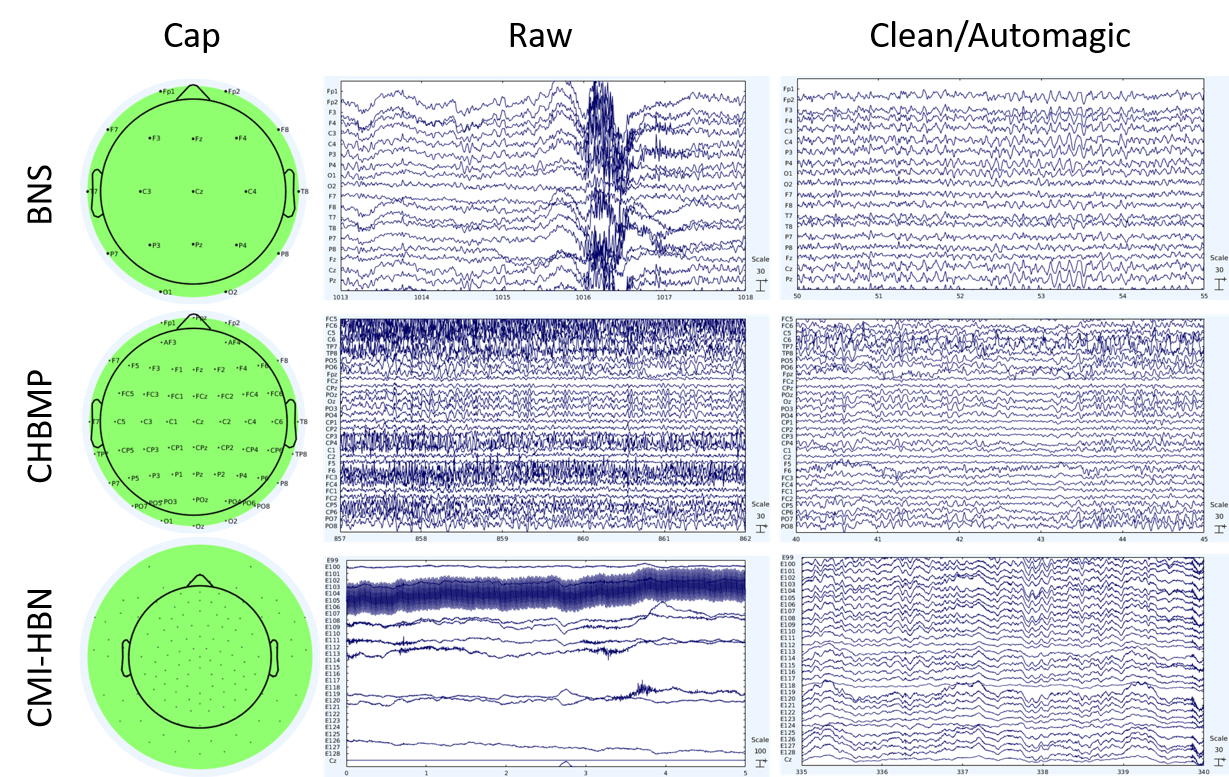
\includegraphics[width=15cm]{pic/palos/data.png}
\caption{谱同构准则测试数据库样本示例。BNS-巴巴多斯营养不良研究脑电数据库,CHBMP-古巴人脑影像数据库,CMI-HBN-美国儿童脑智研究院-人脑网络数据库。BNS和CHBMP的Clean数据是经专家挑选的稳态脑电数据,CMI-HBN Automagic是原始数据经Automagic预处理后的数据。}
\label{fig3}
\end{figure}

从图\ref{fig3}中可以看出,CMI-HBN的原始数据质量最差,含有大量的电极漂移和高频噪声等,经过Automagic预处理后的数据波形看上去较为平稳;CHBMP和BNS的原始数据在某些电极上或数据段内具有明显的伪差,经过专家视觉挑选稳定数据段后,数据非常平稳。


\section{结果与讨论}
\subsection{谱同构指数在数据库上的验证}
我们应用谱同构准则到以上3个数据库中共1525例健康被试的脑电数据。CMI-HBN数据库中的1224例脑电数据一方面来自于儿童和青少年,其次使用了致密的129 GSN型的电极帽,采集到较多的眼电,波动的漂移、高幅、高频数据非常明显,以及包含有很多难以描述类型的伪差。CHBMP中的250例来自整个生命周期的数据,采用较为稀疏的58通道,数据有有少量眼电和部分数据段上波动伪差、某些电极的高阻抗产生的伪差等。BNS中的51例数据来自中年人,采用最为稀疏的19通道,基本上没有采集到眼电,数据段上偶尔呈现因被试头动产生的伪差。我们用谱同构准则用于验证数据质量。对每一例数据,我们首先按照2.56s的长度进行分段,然后按照multi-taper方法计算交叉谱,时间频带宽积为3.5,最大频率为25Hz。 因为CMI的原始数据和Automagic是按照Cz作为参考来计算,我们对CHBMP和BNS的数据都采用Cz参考。
\begin{figure}[!ht]
	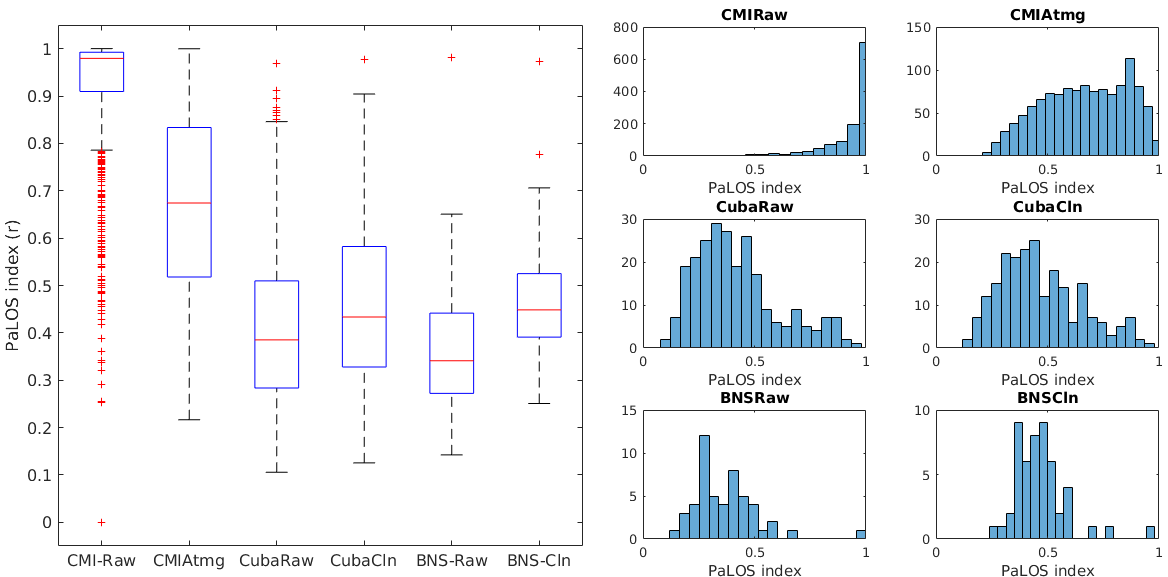
\includegraphics[width=15cm]{pic/palos/comparison.png}
	\caption{谱同构指数数据间对比。CMI-Raw:CMI-HBN原始数据,CMIAtmg:使用Automagic预处理后的CMI-HBN数据,CubaRaw:CHBMP原始数据,CubaCln:CHBMP经专家挑选的稳态数据段,BNSRaw:BNS数据库中原始数据,BNSCln:BNS数据库中经专家挑选的稳态数据段。}
	\label{fig4}
\end{figure}
从图\ref{fig4}中柱状图和直方图可看出,CMI数据库上的谱同构准则(PaLOS index)中值从原始数据时的0.98减小到使用Automagic预处理后的0.66,而Cuba的CHBMP数据库从原始数据的0.38增加到专家挑选的稳态数据段的0.42,Bbds的BNS数据库从原始数据的0.34增加到专家挑选的稳态数据段的0.43。该结果与我们预料的一致,因为CMI的原始数据含有大量冗余的噪声,脑电信号几乎被完全淹没,交叉谱由于噪声高度同构,谱同构指数主要聚集在接近1的位置,使用Automagic进行预处理去除了坏道和明显的伪差,去除伪差后的数据质量因为被试个体差异有所不同,交叉谱反映了更加体现了脑电在大样本被试上的个体差异,谱同构指数下降到中值为0.66但呈现更加离散的分布;Cuba的CHBMP数据库和Bbds的BNS数据库因为采用相同型号的脑电采集设备(Neuronic),而且主试对数据采集的质量控制较好,两个数据库中的原始数据仅具有较少的眼电和时间段较短的明显伪差,另外电极阵列具有更加稀疏的58通道和19通道,不易引入导联间的干扰和因为短路效应引入共线伪差,原始数据的谱同构指数中值在0.34-0.38,甚至低于CMI数据库中预处理后的谱指数中值,由电生理专家视觉挑选出稳态数据段,去除了伪差和非线性非稳态的动力学信息,交叉谱中主要含有的是稳态数据的信息,同构性上升异质性下降,谱同构指数中值增加到0.42-0.43。因此,谱同构指数(PaLOS index)可能有效地表征多通道脑电时间序列预处理的质量和交叉谱的同构异质程度。

\subsection{预处理步骤和参考因素比较}
为了分析谱同构指数在预处理不同步骤和参考之间的差异,我们从CMI数据库中随机挑选10例数据,分别变换原始数据参考为Cz(在Automagic中重参考为鲁棒的平均参考(Rb))、AR和REST再进行Automagic软件分步预处理。从图\ref{fig5}A中显示了三种参考情况下,10例数据的谱同构指数随着Automagic中原始数据(Orig)、坏道挑选(Prep)、滤波(Filt)、眼电回归(Reg)、伪差成分去除(MARA)和坏道插值(Itpl)步骤的变化。 对Itpl步骤后的10例数据,Automagic软件基于脑电时域信息如幅度、方差、坏道比例等质量控制准则,不同参考下的质量控制结果一致,其中被试ID349、904质量为差,被试ID117、948质量为一般,其他数据为良好,。不同参考下的10数据总体上都表明应用坏道挑选(Prep)、眼电回归(Reg)和伪差成分去除(MARA)步骤都会使得谱同构指数上升,相比之下,滤波(Filt)步骤会使得谱同构指数下降。质量为差的349、904数据的谱同构指数在Automagic分步处理中表现了与其它质量为一般或良好的数据谱同构指数不同的分步变化趋势,并且最后在Itpl步骤后的谱同构指数相对其它数据偏高。Prep步骤中去除坏道、Reg步骤中去除眼电、MARA步骤去除更多的伪差成分,特别是MARA步骤的独立成分分析去除的不同伪差成分和眼电、坏道统计学上接近相互独立,代表了原始数据中的异质性,应用这些步骤都使得脑电数据丢失异质信息,从而谱同构指数升高。相比之下,滤波(Filt)后谱同构指数下降,主要是由于应用了带通滤波去除了频率较低(<1Hz)的信息,而低频信息在谱曲线中对应较大的能量,在原始数据中具有较大的幅度,因此除去低频信息丢失了数据的同构信息,虽然丢失的高频信息代表数据的异质性,但因为高频对应幅度较低、谱曲线中能量很小,二者的抵消结果还是数据丢失了更多的同构信息使得谱同构指数下降。
\begin{figure}[!ht]
	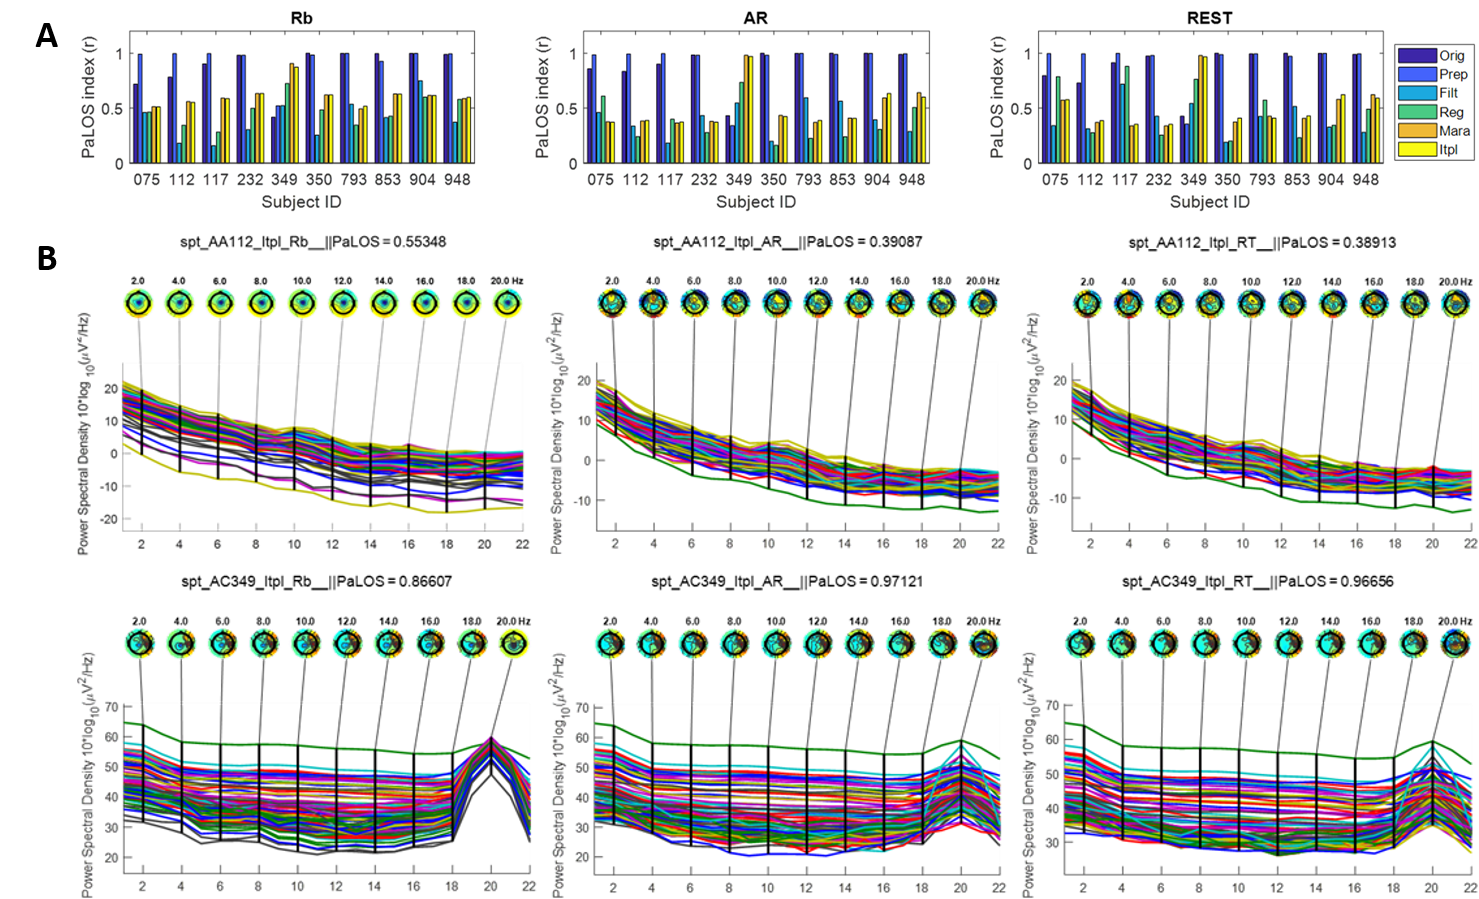
\includegraphics[width=15cm]{pic/palos/step.png}
	\caption{参考与预处理步骤分析。参考Rb:基于Cz的鲁棒平均参考,AR:传统的平均参考,REST:零参考。 A. 谱同构指数随着Automagic主要预处理步骤的变化趋势。 B. 第一行:谱异质的数据112,第二行:谱同构的数据349}
	\label{fig5}
\end{figure}
在图\ref{fig5}B中上下两行分别是一例好的数据112和一例差的数据349在不同参考情况下的的多通道谱曲线和谱地形图分布。对于没有谱同构问题的112,三种参考下的谱同构指数为0.38-0.56,而对于具有谱同构问题的349,三种参考下谱同构指数为0.86-0.97,这说明谱同构指数能够表征实际中是否存在谱同构的问题。不同参考之间比较,对于112,AR和REST比Rb具有更符合谱异质情况的同构指数(0.39<0.55),对于349,AR和REST比Rb具有更符合谱同构情况的同构指数(0.97>0.86),但REST比AR对谱异质的112具有更小的同构指数,AR比REST对谱同构的349具有更大的同构指数。由此可见,总体上,REST和AR下的谱同构指数提供了比Rb参考下的谱同构指数更加符合实际的指数证据,但REST和AR的差异并不明显。

\section{本章小结}
我们分析了脑电数据预处理后数据可能出现谱同构的问题,基于共同主成分分析,提出了一种能够表征脑电谱同构异质程度的指数。结合自动化伪差去除和专家视觉挑选两种预处理方法,我们在不同数据库上进行验证发现这种谱同构指数可能有效地表征多通道脑电时间序列预处理程度。谱同构指数对噪声较强的数据预处理完成后后下降,但在预处理中的分步骤可能会出现上升再下降的趋势。数据的伪差情况不同,分步骤计算的谱同构指数的上升下降趋势就不一致。我们还比较了不同的参考发现参考不会影响自动化分析软件根据时域信息对数据的质量分类,但根据谱的同构异质性,AR和REST比Rb更加符合。总体上,我们希望提出的谱同构准则能作为大样本数据预处理后的一种初筛的准则,避免因为应用很强的预处理算法丢失掉与脑活动有关的信息而出现谱同构的问题。因为脑电的质量控制缺乏真正的基标准,我们希望结合电生理专家去伪差辅助分析,分析更多的数据集找到不同数据质量程度在预处理中谱同构指数的变化趋势,在更多的数据集上借助高性能计算平台进行大样本分析有望找到谱同构准则的阈值范围,实现对数据预处理质量的更加准确的控制。本章中谱同构准则计算方法公开在\href{https://github.com/ShiangHu/PaLOS-index.git}中。